\chapter{Parallel and Perpendicular}
% vectors were not defined beforehand here
A vector is a line or ray with defined length (referred to as magnitude) and direction (given in degrees or radians). Velocity, force, and displacement are all examples of quantities that can be represented as vectors. Vectors are commonly drawn as arrows, where the length of the arrow corresponds to the magnitude and the direction of the arrow shows the direction of the vector.

Understanding how vectors relate to each other—such as being parallel or perpendicular—is fundamental in mathematics and physics.
Two vectors are said to be parallel if they have the same or opposite
direction. In simpler terms, if two vectors are pointing in the same
direction (even if their magnitudes differ), they are considered
parallel. For example, imagine you have a vector representing the
direction and speed of a car moving north. If you have another vector
representing the direction and speed of a different car also moving
north, these vectors are parallel. We have already seen parallel lines 
when talking about parallel circuits, meaning they offer multiple paths 
of flow but don't intersect.\index{parallel}

\begin{center}
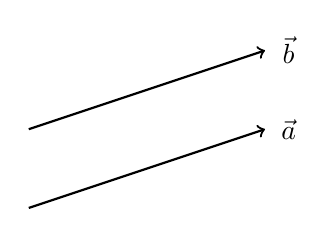
\begin{tikzpicture}[scale=1]
    \draw[thick,->] (0,0) -- (3,1);
    \draw[thick,->] (0,1) -- (3,2);
    \node at (3.3,1) {$\vec{a}$};
    \node at (3.3,2) {$\vec{b}$};
\end{tikzpicture}
\end{center}

On the other hand, if two vectors point are in completely opposite
directions, they are still considered parallel. For example, if one
vector represents a car moving north and the other represents a car
moving south, these vectors are parallel, but in opposite directions.

Perpendicular vectors, as the name suggests, are vectors that
intersect each other at a right angle, forming a 90-degree angle. If
we imagine a sheet of paper, drawing a horizontal vector and a
vertical vector on that paper would create perpendicular vectors. In
this case, the horizontal vector represents left-right direction,
while the vertical vector represents up-down direction. Perpendicular
vectors are often seen in geometric shapes, such as squares and
rectangles, where their sides intersect at right angles. The coordinate planes
are also perpendicular.\index{perpendicular}
\begin{center}
\begin{tikzpicture}[scale=.5]
    % Draw x and y axes
    \draw[->] (-5,0) -- (5,0) node[right] {$x$};
    \draw[->] (0,-5) -- (0,5) node[above] {$y$};
    % Optional: mark the origin
    \node at (0,0) [below left] {O};
\end{tikzpicture}
\end{center}

%FIXME this should be moved to the dot chapter, since we haven't introduced dot product yet. seems out of place here
A fundamental property of perpendicular vectors is that their dot
product is zero. The dot product is a mathematical operation that
measures the extent to which two vectors align with each other. When
two vectors are perpendicular, their dot product is always zero. This
property provides a useful tool for determining whether two given
vectors are perpendicular.

Understanding parallel and perpendicular vectors is essential in
various areas of mathematics and physics. For example, in geometry,
knowledge of perpendicular vectors helps us determine whether lines
are perpendicular or parallel. In physics, vectors can represent
forces, velocities, or displacements, and identifying parallel or
perpendicular vectors aids in analyzing motion and forces acting on
objects.

In summary, parallel vectors have the same or opposite direction,
while perpendicular vectors intersect at a right angle. Recognizing
these relationships between vectors enables us to solve problems
involving geometry, physics, and many other fields. As you delve
deeper into the exciting world of vectors, keep an eye out for
parallel and perpendicular relationships, as they often hold valuable
insights and solutions. We are going to get into graphing these two lines
and their equations in the next chapter!

%FIXME would a section on perpendicular bisectors, alternate interior/exterior angles, and transversals fit here?